\documentclass[12pt,a4paper]{article} 
\usepackage[utf8]{inputenx} 
\usepackage[spanish]{babel} 
\usepackage[left=2cm,right=2cm,top=2cm,bottom=2cm]{geometry}
\usepackage{scrextend}
\usepackage{marvosym}
\usepackage{pifont} % Generación de símbolos especiales
\usepackage{textcomp}
\usepackage{newpxtext}
\usepackage{newpxmath}
\usepackage[T1]{fontenc} % Codificación de salida    
\usepackage{microtype} % Mejoras de microtipografía en la obtención de PDF (sólo para pdflatex)
\usepackage[hyphens]{url} % Para escritura de URL
\urlstyle{sf} % Estilo de URL sin serifas para que tengan un mejor aspecto
\usepackage{tikz}
% Paquetes para obtener un mayor control de las listas
\usepackage{paralist} % Mayor control de listas
\usepackage{multicol} % Elementos en varias columnas
\usepackage[breaklinks]{hyperref}
\usepackage{graphicx}
\usepackage{caption}
\captionsetup[figure]{labelformat=empty}
\author{Julián García Sánchez \and Iván Illán Barraya \and Alejandro Medina Jiménez \and Javier Monescillo Buitrón}
\title{Implementación de un procesador de lenguajes para Autómatas de Moore}
\date{\today}
%%%%%%%%%%%%%%

\begin{document}
	
	\maketitle
	
	\begin{figure}[h]
		\centering
		
\includegraphics[width=0.25
		\linewidth]{img/image004}
		\caption{}
		\label{fig:image004}
	\end{figure}

	\newpage
	\tableofcontents
	\newpage
	
	\section{¿Qué es un autómata de Moore?}
	En Teoría de la computación una \textbf{Máquina de Moore} es un autómata de estados finitos para el cual la salida en un momento dado sólo depende de su estado en ese momento, mientras que la transición al siguiente estado dependerá del estado en el que se encuentre y de la entrada introducida.
	\newline
	El diagrama de estados para una máquina de Moore incluirá una señal de salida para cada estado. \cite{Moore1}
	
	\begin{figure}[h]
		\centering
		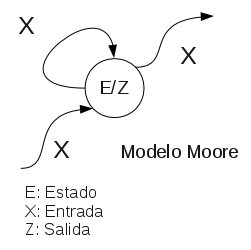
\includegraphics[width=0.5
		\linewidth]{img/Modelo-moore}
		\caption{Ejemplo de Máquina de Moore simple}
		\label{fig:modelo-moore}
	\end{figure}
	
	
	\subsection{Definición formal}
	Una máquina de Moore se define como una 6-tupla:
	\[ Mmor = (S,S_{0},\Sigma,\Lambda,T,G)  \]
	donde definimos los siguientes elementos:
	\begin{itemize}
		\item S: es un conjunto finito de estados.
		\item $S_{0}$: es el estado inicial, y además es un elemento de S.
		\item $\Sigma$: un conjunto finito llamado alfabeto de entrada.
		\item $\Lambda$: un conjunto finito llamado el alfabeto de salida.
		\item $T$ : una función de transición $T: S \times \Sigma \rightarrow S$ mapeando un estado y una entrada al siguiente estado.
		\item $G$ función de salida $G : S \rightarrow \Lambda $ mapeando cada estado al alfabeto de salida.
	\end{itemize}
	\clearpage

	
	\newpage
	\subsection{Ejemplo propuesto}
	Se define una \textit{Máquina de Moore} para regular el tráfico en el siguiente cruce con los cuatro semáforos:
		
	\begin{figure}[h]
		\centering
		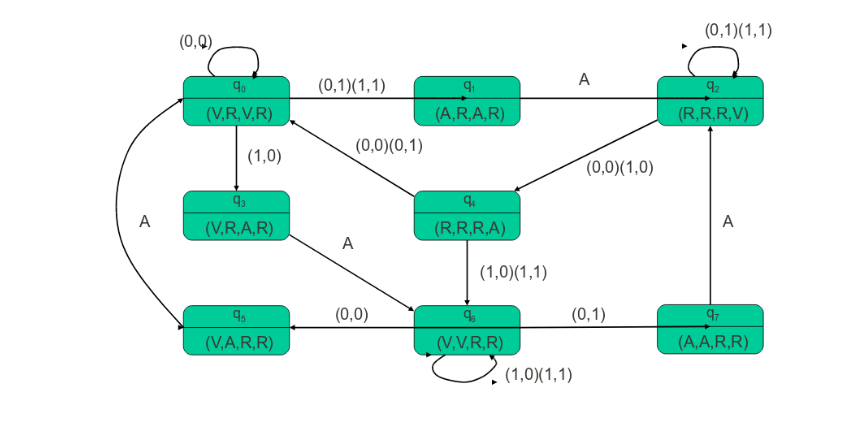
\includegraphics[width=0.4
		\linewidth]{img/4}
		\caption{}
		\label{fig:4}
	\end{figure}

El alfabeto de entrada $\Sigma$: {(0,0),(0,1),(1,0),(1,1)}

	\begin{itemize}
		\item (a,b), donde a es el estado para el sensor $\alpha$ y b para el sensor $\beta$
		\item 0 indica que no hay coches en la cola
		\item 1 indica que hay coches en la cola
	\end{itemize}

El alfabeto de salida $\Lambda$: { ($a_{1},a_{2},a_{3},a_{4}$ donde $a_{i}\epsilon$ (A,V,R) )
	\begin{itemize}
		\item $a_{1}$ es el estado del semáforo 1
		\item $a_{2}$ es el estado del semáforo 2
		\item $a_{3}$ es el estado del semáforo 2
		\item $a_{4}$ es el estado del semáforo 2
	\end{itemize}

	\begin{center}
		\textit{El diagrama de estados sería el siguiente}
	\end{center}

	\begin{figure}[h]
		\centering
		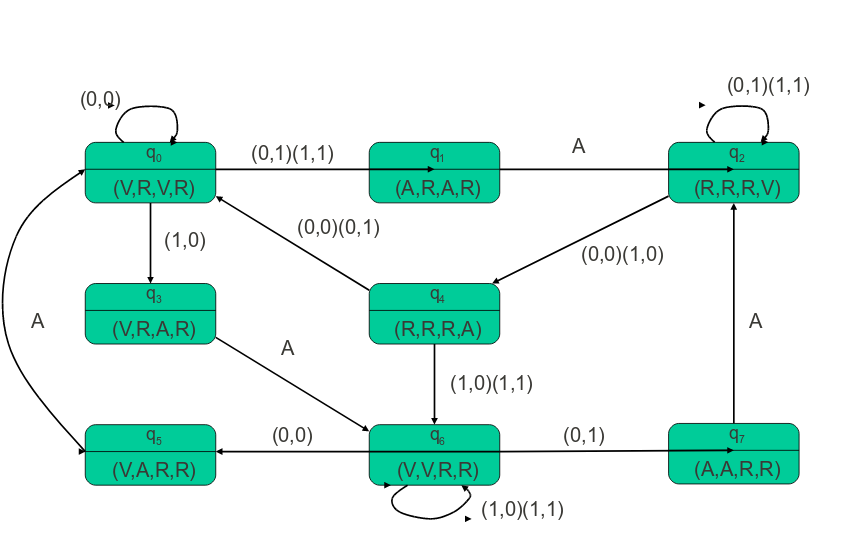
\includegraphics[width=0.7
		\linewidth]{img/3}
		\caption{}
		\label{fig:3}
	\end{figure}

\newpage
\section{Presentación del problema}
La práctica consiste en el diseño de un procesador de lenguajes cuya entrada estará formada por una o varias máquinas de Moore y su salida será código en un lenguaje de alto nivel que lo represente, en nuestro caso Java.
\newline
\newline
Los conocimientos de la materia \textit{Procesadores de Lenguajes} serán útiles en las distintas etapas del proceso, en primer lugar, se necesitará definir el léxico del lenguaje de entrada, la construcción del procesador de lenguajes asociado empleando los diagramas \textbf{tipo T}, el análisis léxico, el análisis sintáctico y por último el análisis semántico.
\newline
\newline
También se desarrollará una tabla de tokens, lexemas y patrones del lenguaje y el EBNF perteneciente al mismo.
\subsection{Lenguaje definido}
El lenguaje \textbf{Moor} que se ha definido consta de dos secciones principales:
\begin{itemize}
	\item Sección de declaración de código
	\item Sección de declaración de autómatas
\end{itemize}
La \textit{zona de declaración de código} es la parte donde se asignará un comportamiento a un código ya predefinido o que se vaya a ejecutar. Por la forma en la que se ha definido el lenguaje, esta zona será como una zona de \textit{imports} típicamente conocida en lenguajes de alto nivel. \newline \newline
La estructura de esta zona es: c$N$ $\#$ \textit{código} $\#$ donde c es el comportamiento, $N$ es el número de comportamiento y los \textbf{tokens} $\#$ son los delimitadores del código. \newline La característica principal de esta zona es que solo se podrán realizar este tipo de declaraciones, ya que en la otra zona solo podremos declarar autómatas.
\begin{center}
	Ejemplo : c1 $\#$ print('hola') $\#$
\end{center}
Respecto a la \textit{zona de declaración de autómatas} se tendrá una serie de palabras que se utilizarán para la definición del autómata. No obstante en esta zona solo se podrán declarar autómatas y las funciones asociadas a los mismos, también, como en cualquier lenguaje de alto nivel, se podrán incluir los clásicos comentarios '//' o '/$\ast$ Texto comentario '$\ast$/'.
\newline \newline
Será posible la declaración de múltiples autómatas en el fichero de prueba, además, se indicará en una tabla todos los campos que son imprescindibles para la realización del mismo.
Cualquier otro carácter introducido en el fichero de prueba será considerado como error.

\subsection{Tabla Token-Acción}
\clearpage
\begin{center}
\begin{tabular}{|c|c|}
	\hline 
	\textbf{Token} & \textbf{Acción} \\ 
	\hline 
	moore & Función para declarar un autómata seguido de un nombre   \\
	& que se escribirá entre llaves $\{\}$ moore Ejemplo $\{\}$\\
	\hline 
	estados & Indica la cantidad de estados totales que tendrá el autómata  \\
	& puede ser un único estado o varios separados por ',' estados q0,q1;\\ 
	\hline 
	estado\_in & Se selecciona un único estado inicial  \\ 
	& que tendrá que estar en los estados anteriores estado\_in q0; \\
	\hline 
	alf\_in & La entrada o eventos del autómata que hará posible las transiciones\\
	& entre estados, único o entre comas ',' alf\_in a,b,c;\\
	\hline 
	alf\_out &  La salida o comportamientos del autómata  \\
	& y tendrán que ser coincidentes con \\ 
	& la zona de declaración de comportamientos, \\
	&  escrito un identificador único o entre comas ',' \\
	\hline
	transicion & Será un tipo de función que se escribirá entre llaves $\{\}$, \\
	& y permitirá que se transite mediante una entrada de un estado a otro: \\ 
	& (<estado\_origen>, entrada, <estado\_destino>); \\
	& se podrán indicar varias mediante el uso de comas ',' \\
	\hline 
	comportamiento & Será un tipo de función que se escribirá entre llaves $\{\}$,   \\ 
	& y permite asignar a un estado un comportamiento: \\
	& (<estados>,<comportamiento>); \\
	& se podrán indicar varios mediante el uso de comas ','\\
	\hline  
\end{tabular} 
\end{center}
Notese que para cerrar una sentencia es necesario de indicar al final de dicha sentencia el carácter ';', esto no es necesario para las funciones \textit{moore}, \textit{transicion} y \textit{comportamiento}.
\subsection{Ejemplo autómata completo}
\begin{center}
\begin{figure}[h]
	\centering
	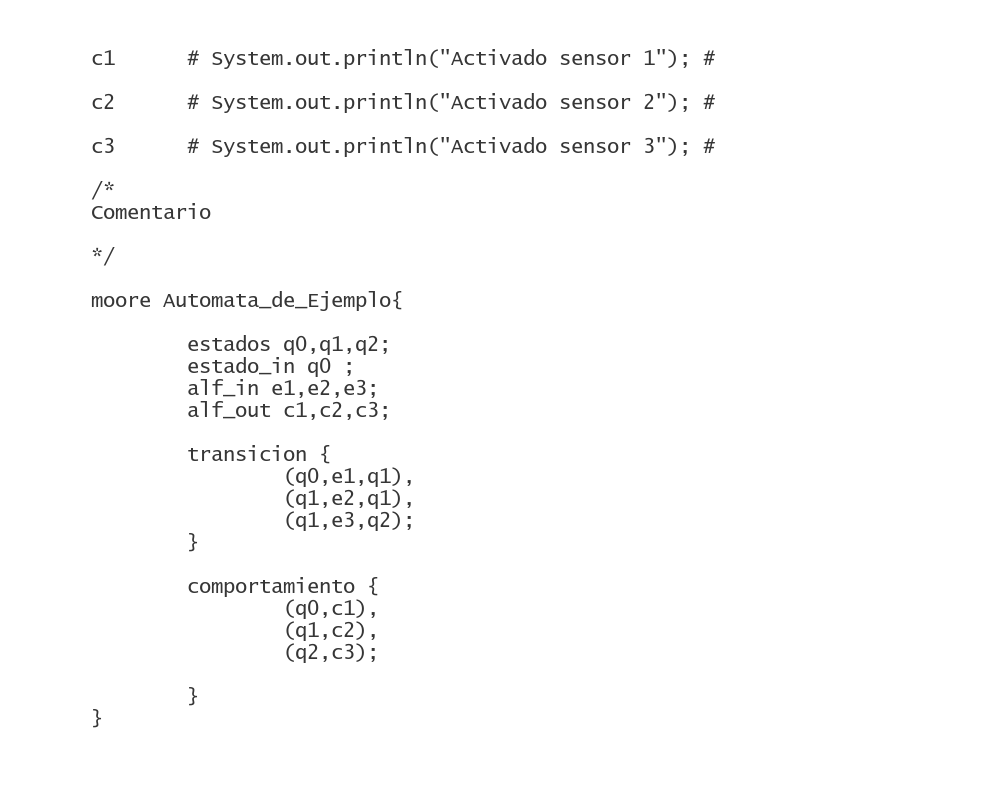
\includegraphics[width=0.75\linewidth]{img/ejemplo}
	\caption{}
	\label{fig:aut}
\end{figure}

	\end{center}
	\section{EBNF}
			\begin{center}
			\begin{tabular}{lcl}
	

				PROGRAMA & ::= & DEC$\_$COMP AUTOMATA $\{$AUTOMATA$\}$ \\ 
				 
				
				DEC$\_$COMP & ::= &CMP  CODIGO $\{$ CMP CODIGO $\}$ \\ 
			
				CODIGO 	&::= &'$\#$' ASCII '$\#$' \\ 
				
				AUTOMATA & ::= & \textbf{moore} ID CUERPO$\_$AUTOMATA \\
				
			
				CUERPO$\_$AUTOMATA	& ::= & $'\{'$ ESTADOS ESTADO$\_$INI ALF$\_$IN  \\ 
				
					& &  ALF$\_$OUT TRANSICION COMPORTAMIENTOS $'\}'$ \\ 
				
				ESTADOS	& ::= &   \textbf{estados} $\{$ ID ',' $\}$ ID ';'\\ 
				
				 ESTADO$\_$INI &::= & \textbf{estado$\_$in} ID ';'\\ 
				 
				ALF$\_$IN &::= & \textbf{alf$\_$in}  $\{$ EVENTOS ',' $\}$ EVENTOS ';' \\ 
				
				ALF$\_$OUT & ::= &\textbf{alf$\_$out}  $\{$ CMP ',' $\}$ CMP ';'  \\ 
				
				TRANSICION 	 & ::= & \textbf{transicion} $'\{'$ TRANSICION$\_$DEF $\{$ ',' TRANSICION$\_$DEF  $\}$ ';' $'\}'$ \\ 
				
				TRANSICION$\_$DEF & ::= & '(' ID ',' ID ',' ID ')' \\ 
			
				
				COMPORTAMIENTOS	 & ::= &  \textbf{comportamientos} $'\{'$ COMP$\_$DEF $\{$ ',' COMP$\_$DEF $\}$ ';' $'\}'$\\ 
				
				COMP$\_$DEF &  ::= & '(' ID ',' ID ',' ID ')' \\ 
				
				
				CMP  & ::= & 'c'NUMEROS \\ 
				
				NUMEROS &::= & 0 | 1 | .. | 9 \\ 
				
				COMENTARIOS & ::=  & $'/\ast'$ ASCII $'\ast/'$ \\
				
				
			\end{tabular} 	
		\end{center}
	
	
	\section{Tablas de Tokens}
		
	\begin{center}
		\begin{tabular}{|c|c|c|}
			\hline 
			\textbf{Token} & \textbf{Lexema} & \textbf{Patrón} \\ 
			\hline 
			moore & moore & m$\cdot$o$\cdot$o$\cdot$r$\cdot$e  \\ 
			\hline 
			estados &estados & e$\cdot$s$\cdot$t$\cdot$a$\cdot$d$\cdot$o$\cdot$s \\ 
			\hline 
			estado$\_$in & estado$\_$in & e$\cdot$s$\cdot$t$\cdot$a$\cdot$d$\cdot$o$\cdot$$\_$$\cdot$i$\cdot$n \\ 
			\hline 
			alf$\_$in	& alf$\_$in & a$\cdot$l$\cdot$f$\cdot$$\_$i$\cdot$n \\ 
			\hline 
				alf$\_$out	& alf$\_$out & a$\cdot$l$\cdot$f$\cdot$$\_$o$\cdot$u$\cdot$t \\ 
			\hline 
				transicion	& transicion & t$\cdot$r$\cdot$a$\cdot$n$\cdot$s$\cdot$i$\cdot$c$\cdot$i$\cdot$o$\cdot$n \\ 
			\hline 
				comportamiento	& comportamiento & c$\cdot$o$\cdot$m$\cdot$p$\cdot$o$\cdot$r$\cdot$t$\cdot$a$\cdot$m$\cdot$i$\cdot$e$\cdot$n$\cdot$t$\cdot$o \\ 
			\hline 
			Paréntesis abierto	& ( & ( \\ 
			\hline 
			Paréntesis cerrado	& ) & ) \\ 
			\hline 
			Llave abierta	& $\{$ & $\{$ \\ 
			\hline 
			Llave cerrada	& $\}$ & $\}$ \\ 
			\hline 
			Punto y coma	& ; & ; \\ 
			\hline 
			Coma	& , &  , \\ 
			\hline
			Asterisco barra & $\ast/$  & $\ast$$\cdot/$ \\ 
			\hline 
			Barra asterisco & $/\ast$  &  $/$$\cdot$$\ast$ \\ 
			\hline  
			ID	& hola  & [A-Za-z][A-Zaz0-9$\_$]* \\ 
			\hline 
			CMP	& c1 & c[1-9][0-9]* \\ 
			\hline
		    CODIGO	& $\#$codigo aquí $\#$  & $\#$$\cdot$ codigo aquí $\cdot$$\#$\\ 
			\hline
			
		
	
		\end{tabular} 	
	\end{center}
	\newpage
	\section{¿Cómo se va a construir el procesador del lenguaje diseñado?}
	En el siguiente diagrama tipo T se explica el funcionamiento del procesador que se pretende implementar, tomamos \textbf{ Moor } como lenguaje fuente, y Java como lenguaje objeto, y además el lenguaje que implementa es Java, es decir, nuestro compilador compila a Java, y esta escrito a Java. 
	\newline
	Para utilizar ese compilador, utilizamos un compilador auxiliar, que está escrito en código máquina para dar lugar a bytecode, el típico archivo \textbf{.class} que generamos al compilar el archivo \textbf{.java}.
	\newline
	Por último tenemos que compilar el bytecode, con un compilador que acepta bytecode escrito en código máquina.
	
	\begin{figure}[h]
		\centering
		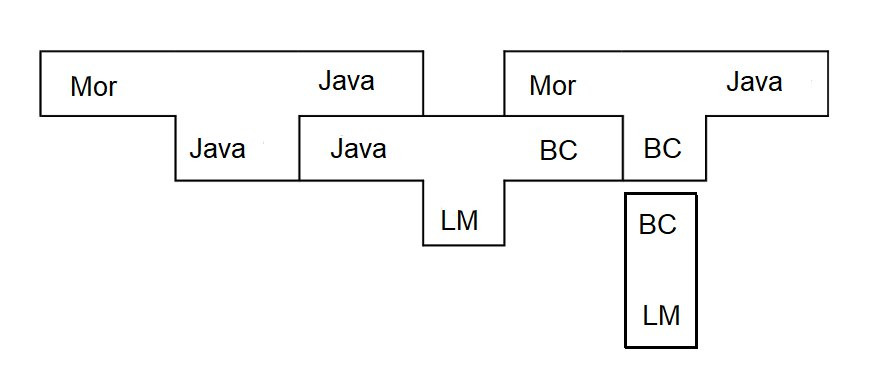
\includegraphics[width=0.7
		\linewidth]{img/photo5978652419892031524}
		\caption{Diagrama tipo T asociado}
		\label{fig:photo5978652419892031524}
	\end{figure}
	
	\section{Estructura del procesador de lenguajes}
	Siguiendo la estructura que se ha utilizado en clase, tenemos la siguiente organización:
	\begin{figure}[h]
		\centering
		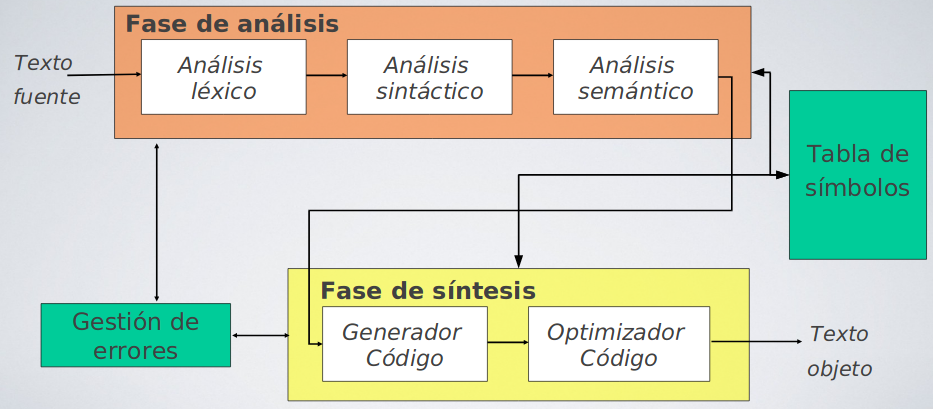
\includegraphics[width=0.7\linewidth]{img/estructura}
		\caption{}
		\label{fig:estructura}
	\end{figure}
	
	El procesador de lenguajes que se va a construir seguirá una estructura similar salvo por el bloque de la fase de síntesis, ya que no se ha visto en la asignatura.

	
	\clearpage
	Se procederá a la construcción de la fase de análisis que consta de las siguientes etapas:
	\begin{itemize}
		\item Análisis léxico
		\item Análisis sintáctico
		\item Análisis semántico
	\end{itemize}
	\section{Analizador léxico}
	\subsection{Jflex}
	\subsection{ANTLR}
	\section{Analizador sintáctico}
	\subsection{CUP}
	\subsection{ANTLR}
	
	\section{Analizador semántico}
	\clearpage
	
	\begin{thebibliography}{99}
		\bibitem{Moore1} Autómatas de Moore \url{https://es.wikipedia.org/wiki/M%C3%A1quina_de_Moore}
	
	\end{thebibliography}
	
	
	
	
	
\end{document}\grid
